\section{The Pulsar/\Actitle{PWN} System}
\seclabel{pulsar_pwn_system}

\subsection{Neutron Star Formation}

As was discussed in \secref{astrophysical_sources}, pulsars, 
\acp{PWN},
and supernova remnants are all the end products of supernovas.  When a
star undergoes a supernova, the ejecta forms a supernova rememant.  If the
remaining stellar core has a mass above the Chandrasekhar limit,
then the core's electron degeneracy pressure cannot counteract the core's
gravitational force and the core will collapse into a neutron star.
The Chandrasekhar mass limit can be
approximated as \citep{chandrasekhar_1931_maximum-ideal}
\begin{equation}
  \MassChandrasekhar \approx 
  \frac{3\sqrt{2\pi}}{8}
  \left(\frac{\hbar\speedoflight}{\gravitationalconstant}\right)^{3/2}
  \left[
  \left(\frac{\NumberProtons}{\NumberNucleons}\right)
  \frac{1}{\MassHydrogen^2}
  \right]
\end{equation}
where $\hbar$ is the reduced Planck constant, \speedoflight is the
speed of light, \gravitationalconstant is the gravitational constant,
\MassHydrogen is the mas sof hydrogen, \NumberProtons is the
number of protons, \NumberNucleons is the number of nucleons, and
\solarmass is the mass of the sun.  This formula can be found in
\citep{carroll_2006_introduction-modern}.
More precisely, $\MassChandrasekhar = 1.44 \solarmass$.

Because neutron starts are supported by a
neutron degeneracy pressure,
the radius of a neutron star can be approximated as
\begin{equation}
  \RadiusNeutronStar \approx \frac{(18 \pi)^{2/3}}{10}
  \frac{\hbar^2}{\gravitationalconstant \MassNeutronStar^{1/3}}
  \left(\frac{1}{\MassHydrogen}\right)^{8/3}
\end{equation}
This formula can be found in \citep{carroll_2006_introduction-modern}.
The canonical radius for neutron stars is $\sim 10\unitspace\km$.

In these very dense enviroments, the protons and electrons in the neutron
star form into neutrons through inverse $\beta$ decay:
\begin{equation}
  \proton^\positive + \electron^\negative 
  \processarrow \neutron + \electronneutrino.
\end{equation}

But if a neutron star had a sufficiency large mass, the graviational
force would overpower the neutron degeneracy pressure and the
object would collapse into a black hole. The maximum mass of a
neutron star is unknown because it depends on the equation of state
inside the star, but is comonly predicted to be $\sim 2.5\solarmass$
Recently, a pulsar with a mass of $\sim 2\solarmass$ was discovered
\citep{demorest_2010_two-solar-mass-neutron}, constrainging
theories of the equation of state.



\todo[inline]{3 Types of pulsars (rotationalally powered pulsars,
magnetars, accretion powered pulsars,}

\subsection{Pulsar Evolution}

% Good discussion of PWN physics with some simple formulas: 
%   ``The Evolution and Structure of Pulsar Wind Nebulae''
%   Bryan M. Gaensler and Patrick O. Slane


% good discussion of radius of termination shock in: kargaltsev_2008_pulsar-nebulae

% Another review paper (looks to describe pulsar modeling):
%  ``High Energy Studies of Pulsar Wind Nebulae''
%     Patrick Slane

% Also, Adam Van Etten's thesis: 1.1 Pulsar Wind Nebula Structure

% Good reference: ``Carroll and Ostlie'' page 593

% good refernce on PWN physics: \cite{fuste_2007_g-ray-observations}

\begin{figure}[htpb]
  \begin{center}
    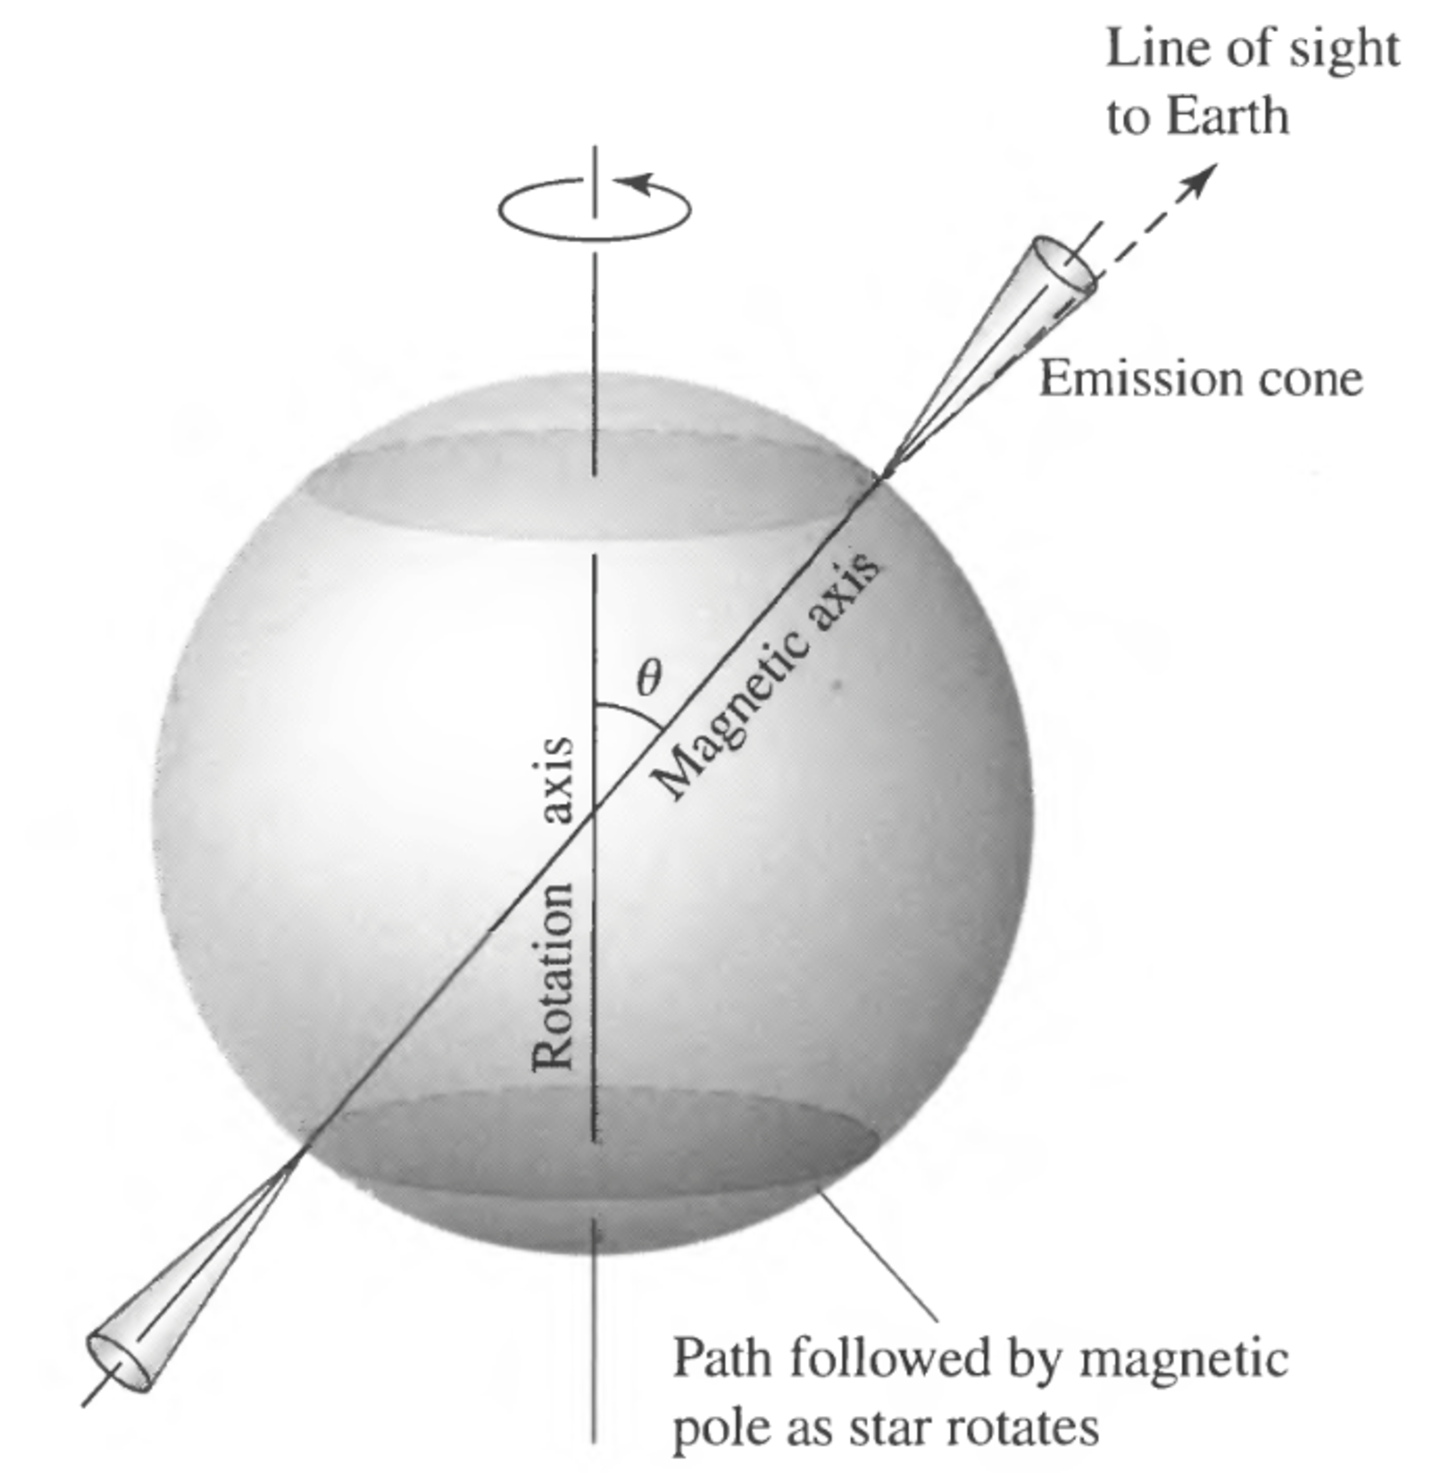
\includegraphics[width=\textwidth]{chapters/introduction/figures/pulsar_model.pdf}
  \end{center}
  \caption{The simplest model of a puslar. This
  figure is taken from \citep{carroll_2006_introduction-modern}.
  }
  \figlabel{pulsar_model}
\end{figure}

The simplest model of a pulsar is that it is a rotating dipole magnet
with the rotation axis and the magnetic axis offset by an angle
$\PulsarRotationAngle$.
A diagram of this model is shown in \figref{pulsar_model}.
The energy output from the pulsar is
then assumed 
to come from rotational kintetic energy stored in
the netutron star which is released as the pulsar
spins down. 

Both the period \period and the period derivative
$\perioddot=d\period/d\time$ can be directly observed for a pulsar.
Except in a few millisecond pulsars which are being sped up
through accreition (see for example \cite{falanga_2005_integral-observations}),
pulsars are slowing down ($\perioddot<0$).

We write the rotational kinetic energy as
\begin{equation}\eqnlabel{rotational_energy}
  \energyrotational = \tfrac{1}{2} I \angularfrequency^2
\end{equation}
where $\angularfrequency = 2\pi/\period$ is
the angular frequency of the pulsar and
\momentofinertia is the moment of inertia.

For a uniform sphere,
\begin{equation}
  \momentofinertia = \frac{2}{5} M R^2
\end{equation}
Assuming a canonical pulsar as was described in \secref{pulsar_pwn_system},
we find a canonical moment of inertia of 
$\momentofinertia=10^{45}\unitspace\gram\unitspace\cm^{-2}$.

We make the conection between the pulsar's spin-down
energy and the rotational kinetic energy as $\energydot = -
\derivative\energyrotational/\dtime$. Using this,
\eqnref{rotational_energy} can be rewritten as
\begin{equation}\eqnlabel{edot_from_rotation}
  \energydot = I \angularfrequency \angularfrequencydot
\end{equation}

It is believed that as the pulsar spins down, the this rotational energy
is released as pulsed electromagnetic radiation and also as a wind of
electrons and positrons accelerated in the magnetic field of the pulsar.

If the pulsar were a pure dipole magnet, its radiation would be
described as \citep{gunn_1969_magnetic-dipole}
\begin{equation}\eqnlabel{edot_pure_dipole}
  \energydot \propto \frac{\MagneticField^2 \PulsarRadius^6 
  \angularfrequency^4 \sin^2\PulsarRotationAngle}{
  \speedoflight^3}
\end{equation}

Combinding equationts \eqnref{edot_from_rotation} and
\eqnref{edot_pure_dipole}, we find that for a pure dipole magnet,
$\angularfrequencydot \propto \angularfrequency^3$.
In reality, the breaking index of :q

\begin{itemize}
  \item ``.All these six braking indices are smaller than
the value (n = 3) predicted by pure dipole magnetic field
configuration, which may suggest that other spin-down
torques do work besides the energy loss via dipole
radiation'' -- \url{http://vega.bac.pku.edu.cn/rxxu/publications/P/yxz07.pdf}
\end{itemize}


\begin{itemize}
  \item ``though n has only been confidently measured for five pulsars,
  in each case falling in the range 2 < n < 3 (Livingstone et al. (2007)
  and references therein).'' -- Adam Van Etten's thesis
\end{itemize}

We conventionally assume that the period and period derivative are related
by the equation
\begin{equation}\eqnlabel{angular_frequency_derivative_relation}
  \angularfrequencydot \propto \angularfrequency^\breakingindex
\end{equation}
where $\angularfrequency=2\pi/\period$, and $\breakingindex$
is the pulsar breaking index. 

\begin{itemize}
\item ``The braking index is the power to which the slowdown in angular
velocity occurs, and is defined as:
  \begin{equation}
    n = \frac{\period \perioddotdot}{\perioddot} + 2
  \end{equation}
  '' -- keogh\_2010\_search-pulsar
\end{itemize}

Equation \eqnref{angular_frequency_derivative_relation} is
a Bernoulli differential equation which can be integrated to solve for time

\begin{equation}
  T = \frac{\period}{(\breakingindex-1) |\perioddot|}
  \left(
  1-\left(\frac{\period_0}{\period}\right)^{(\breakingindex-1)}
  \right)
\end{equation}

\begin{itemize}
  \item TODO: cite Manchester \& Taylor 1977
\end{itemize}



\begin{equation}
  \pulsarage = \period/2\perioddot
\end{equation}


\begin{itemize}
  \item What is a typical moment of inertia, typical dE/dT
  \item What fraction of pulsar energy is released observationally
\end{itemize}

\subsection{Pulsar Magnetosphere}

\subsection{Pulsar Wind Nebulae}

\begin{itemize}
  \item ``Following this discovery, a theoretical understanding was
  soon developed in which the central pulsar generates a magnetized
  particle wind, whose ultrarelativistic electrons and positrons radiate
  synchrotron emission across the electromagnetic spectrum (Pacini \&
  Salvati 1973, Rees \& Gunn 1974). The pulsar has steadily released
  about a third of its total reservoir of ???? ergs
  of rotational energy into its surrounding nebula over the last 950
  years. This is in sharp contrast to shell-like SNRs, in which the
  dominant energy source is the ??? ergs of kinetic energy
  released at the moment of the original SN explosion.''  -- \cite{gaensler_2006_evolution-structure}
  \item 
    % described in Adam Van Etten's thesis
    What is terminaltion shock of \glspl{PWN}.
  \item 
    How is pulsar outflow accelerated at shock?
\end{itemize}



\begin{itemize}
  \item Discuss termination shock (i.e. section 3.3.2 of dalton\_2011\_identication-gamma-ray
  \item The radius of the termination shock is
    \begin{equation}
      \radiusterminationshock = \sqrt{\frac{\energydot}{\tfrac{4}{3}\pi \pressureISM \speedoflight}}
    \end{equation}

\end{itemize}

\todo[inline]{Discuss pulsar evolution ``The Evolution and Structure of
Pulsar Wind Nebulae'' -- Bryan M. Gaensler and Patrick O. Slane}

\todo[inline]{Describe Mattana's work on \glspl{PWN}: ``On the evolution of
the Gamma- and X-ray luminosities of Pulsar Wind Nebulae''}

